\documentclass[10pt,aspectratio=169]{beamer}

\usetheme[progressbar=frametitle,numbering=fraction]{metropolis}

\usepackage[T1]{fontenc}
\usepackage[utf8]{inputenc}
\usepackage[brazil]{babel}
\usepackage[sfdefault]{FiraSans}
\usepackage{FiraMono}
\usepackage{booktabs}
\usepackage{graphicx}

\graphicspath{{../relatorio/figures/}}

\definecolor{VerdeDepois}{HTML}{12805A}
\definecolor{LaranjaAntes}{HTML}{B5651D}
\definecolor{FundoTitulo}{HTML}{1B3A33}

\setbeamercolor{frametitle}{bg=FundoTitulo, fg=white}
\setbeamercolor{progress bar}{fg=VerdeDepois, bg=VerdeDepois!25}
\setbeamercolor{title separator}{fg=VerdeDepois}
\setbeamercolor{alerted text}{fg=LaranjaAntes}
\setbeamercolor{example text}{fg=VerdeDepois}

\newcommand{\antes}[1]{{\color{LaranjaAntes}#1}}
\newcommand{\depois}[1]{{\color{VerdeDepois}#1}}

\title{Adaptação de Modelos de Linguagem para o Domínio Público Piauiense}
\subtitle{Questões 01 a 06 \,\textbullet\, Tópicos em Inteligência Artificial \,\textbullet\, 2026.1}
\author{Allycia \and Heverton \and Izaías \and Oscar}
\institute{Departamento de Computação, UFPI \\ Professor: Raimundo Santos Moura}
\date{}

\begin{document}

\maketitle

\begin{frame}{O trabalho em uma página}
  Seis questões sobre adaptar e usar com segurança modelos de linguagem no domínio do Piauí. O núcleo (Q1--Q3) adapta o \textbf{Qwen2.5-0.5B} com três técnicas, medindo tudo \antes{antes} e \depois{depois}:
  \begin{itemize}
    \item \textbf{Q1, Pré-treino continuado:} 71.431 diários oficiais do DOMPI-2025, sem rótulos
    \item \textbf{Q2, SFT completo:} 1.977 pares de instrução gerados do docentesDC, todos os pesos
    \item \textbf{Q3, QLoRA:} mesmos dados da Q2, modelo em 4 bits, só 0,44\% dos parâmetros
  \end{itemize}
  \vfill
  \begin{center}
    \small
    \begin{tabular}{@{}l l r r r@{}}
      \toprule
      \textbf{Experimento} & \textbf{Dataset} & \textbf{Params. treinados} & \textbf{Tempo} & \textbf{VRAM} \\
      \midrule
      Q1 Pré-treino  & DOMPI-2025 & 494M (100\%)   & 4h23   & 10,60 GB \\
      Q2 SFT completo & docentesDC & 494M (100\%)   & 11 min & 9,77 GB \\
      Q3 QLoRA        & docentesDC & 2,16M (0,44\%) & 18 min & 1,77 GB \\
      Extra: QLoRA 1.5B & docentesDC & 4,36M (0,28\%) & 26 min & 2,75 GB \\
      \bottomrule
    \end{tabular}
  \end{center}
  \vfill
  Q1--Q3 em \textbf{uma única sessão de GPU T4 (Kaggle), 5h34}. As Questões \textbf{04} (destilação), \textbf{05} (RAG) e \textbf{06} (guardrails) estendem o estudo, com modelos, ferramentas e ambientes próprios.
\end{frame}

\begin{frame}{Metodologia comum}
  \begin{columns}[T]
    \column{0.5\textwidth}
      \textbf{Dados}
      \begin{itemize}
        \item DOMPI-2025: 77.337 documentos OCR do Diário Oficial dos Municípios do PI
        \item docentesDC: 13.762 registros de 19 professores do DC/UFPI (slides, artigos, código)
      \end{itemize}
    \column{0.5\textwidth}
      \textbf{Protocolo}
      \begin{itemize}
        \item Mesmas métricas: perplexidade, entropia cruzada, acurácia de tokens
        \item Avaliação em conjunto reservado, geração determinística
        \item Q2/Q3: perda e métricas só nos \textbf{tokens de resposta} (máscara no prompt)
      \end{itemize}
  \end{columns}
  \vfill
  \begin{alertblock}{Cuidado de leitura}
    Q1 mede a sequência completa; Q2 e Q3 medem só a resposta. Escalas não são comparáveis entre questões, apenas as variações relativas.
  \end{alertblock}
\end{frame}

\section{Questão 01: Pré-Treino Continuado}

\begin{frame}{Q1: o modelo aprendeu o domínio}
  \begin{center}
    
\includegraphics[width=0.92\textwidth]{q1_metricas.png}
  \end{center}
  \begin{itemize}
    \item Perplexidade: \antes{21,78} para \depois{2,09} (queda de 90,4\%)
    \item Acurácia de tokens: \antes{42,25\%} para \depois{82,03\%}
    \item Perda de validação caindo até o fim (0,842 na época 1; 0,736 na época 2): sem overfitting
  \end{itemize}
\end{frame}

\begin{frame}{Q1: benchmark de 25 perguntas, antes e depois}
  \begin{columns}[T]
    \column{0.42\textwidth}
      \small
      \begin{tabular}{@{}l c c c@{}}
        \toprule
        & \textbf{Exato} & \textbf{Parcial} & \textbf{Erro} \\
        \midrule
        \antes{Base}     & 0 & 5 & 20 \\
        \depois{Treinado} & \textbf{6} & \textbf{7} & \textbf{12} \\
        \bottomrule
      \end{tabular}
      \vspace{1em}
      \begin{itemize}
        \item Acertos exatos, caractere por caractere: CNPJ e CEP de Aroazes, CNPJ de Assunção do Piauí, CEP de Anísio de Abreu
        \item Risco novo: \alert{alucinação plausível} (CNPJ bem formatado, porém errado)
      \end{itemize}
    \column{0.56\textwidth}
      
\includegraphics[width=\textwidth]{q1_benchmark_qa.png}
  \end{columns}
\end{frame}

\begin{frame}{Q1: o mesmo prompt, dois modelos}
  \textit{``EXTRATO DE CONTRATO. Contratante: Prefeitura Municipal de''}
  \vspace{0.5em}
  \begin{exampleblock}{\antes{Base (antes)}}
    ``São Pedro, do Distrito Federal, e do Município de Ipiranga\ldots{} O Tribunal Regional Federal da 4ª Região\ldots'' \hfill {\footnotesize alucina, fora do domínio}
  \end{exampleblock}
  \begin{exampleblock}{\depois{Treinado (depois)}}
    ``São João do Arraial-PI, CNPJ n. 01.612.609/0001-84. Contratado: A. C. GOMES COMÉRCIO DE MATERIAIS ESPORTIVOS E CONSTRUÇÃO LTDA\ldots'' \hfill {\footnotesize município real, CNPJ verdadeiro}
  \end{exampleblock}
  \vfill
  O modelo treinado cita a Lei 14.133/2021, municípios reais do Piauí e reproduz a estrutura de portarias e extratos.
\end{frame}

\section{Questão 02: Pós-Treino com SFT}

\begin{frame}{Q2: dados verificáveis por construção}
  Sem modelo gerador disponível, toda resposta é derivada programaticamente do próprio dado: nada de alucinação como gabarito.
  \begin{columns}[T]
    \column{0.55\textwidth}
      
\includegraphics[width=\textwidth]{q2_pipeline_funil.png}
    \column{0.43\textwidth}
      \small
      \textbf{Cinco tipos de tarefa}
      \begin{itemize}
        \item A: atribuição de origem (700)
        \item B: continuação do trecho (500)
        \item C: tema do trecho (377)
        \item D: fatos sobre o dataset (200)
        \item E: material com código (200)
      \end{itemize}
      \vspace{0.5em}
      10\% dos registros de cada professor reservados antes da geração: a avaliação usa só trechos nunca vistos.
  \end{columns}
\end{frame}

\begin{frame}{Q2: resultados e um episódio de overfitting}
  \begin{columns}[T]
    \column{0.5\textwidth}
      
\includegraphics[width=\textwidth]{q2_curva_loss.png}
    \column{0.48\textwidth}
      \begin{itemize}
        \item Perplexidade (resposta): \antes{14,57} para \depois{7,49} (queda de 48,6\%)
        \item Acurácia de tokens: \antes{51,28\%} para \depois{63,84\%}
        \item Validação sobe na época 3 (0,914 para 0,992): com 1.728 exemplos, o modelo começa a decorar
        \item A seleção automática do melhor checkpoint restaurou a época 2
      \end{itemize}
  \end{columns}
\end{frame}

\begin{frame}{Q2: o modelo passou a saber o que não sabia}
  \textit{``Quem é o professor com mais material no dataset docentesDC?''}
  \begin{exampleblock}{\antes{Base (antes)}}
    ``O professor com mais material no dataset docentesDC é o professor que possui mais materiais, sendo ele o profe\ldots'' \hfill {\footnotesize resposta circular}
  \end{exampleblock}
  \begin{exampleblock}{\depois{SFT (depois)}}
    ``O professor com mais material no dataset docentesDC é Raimundo Santos Moura.'' \hfill {\footnotesize correto}
  \end{exampleblock}
  \vfill
  Nas 10 perguntas de avaliação: base \antes{0 acertos}; SFT \depois{6 acertos, 2 parciais, 2 erros}, incluindo atribuir trechos inéditos ao professor correto.
\end{frame}

\section{Questão 03: Pós-Treino com QLoRA}

\begin{frame}{Q3: adaptação com 0,44\% dos parâmetros}
  \begin{columns}[T]
    \column{0.52\textwidth}
      
\includegraphics[width=\textwidth]{q3_lora_params.png}
      \vspace{0.3em}
      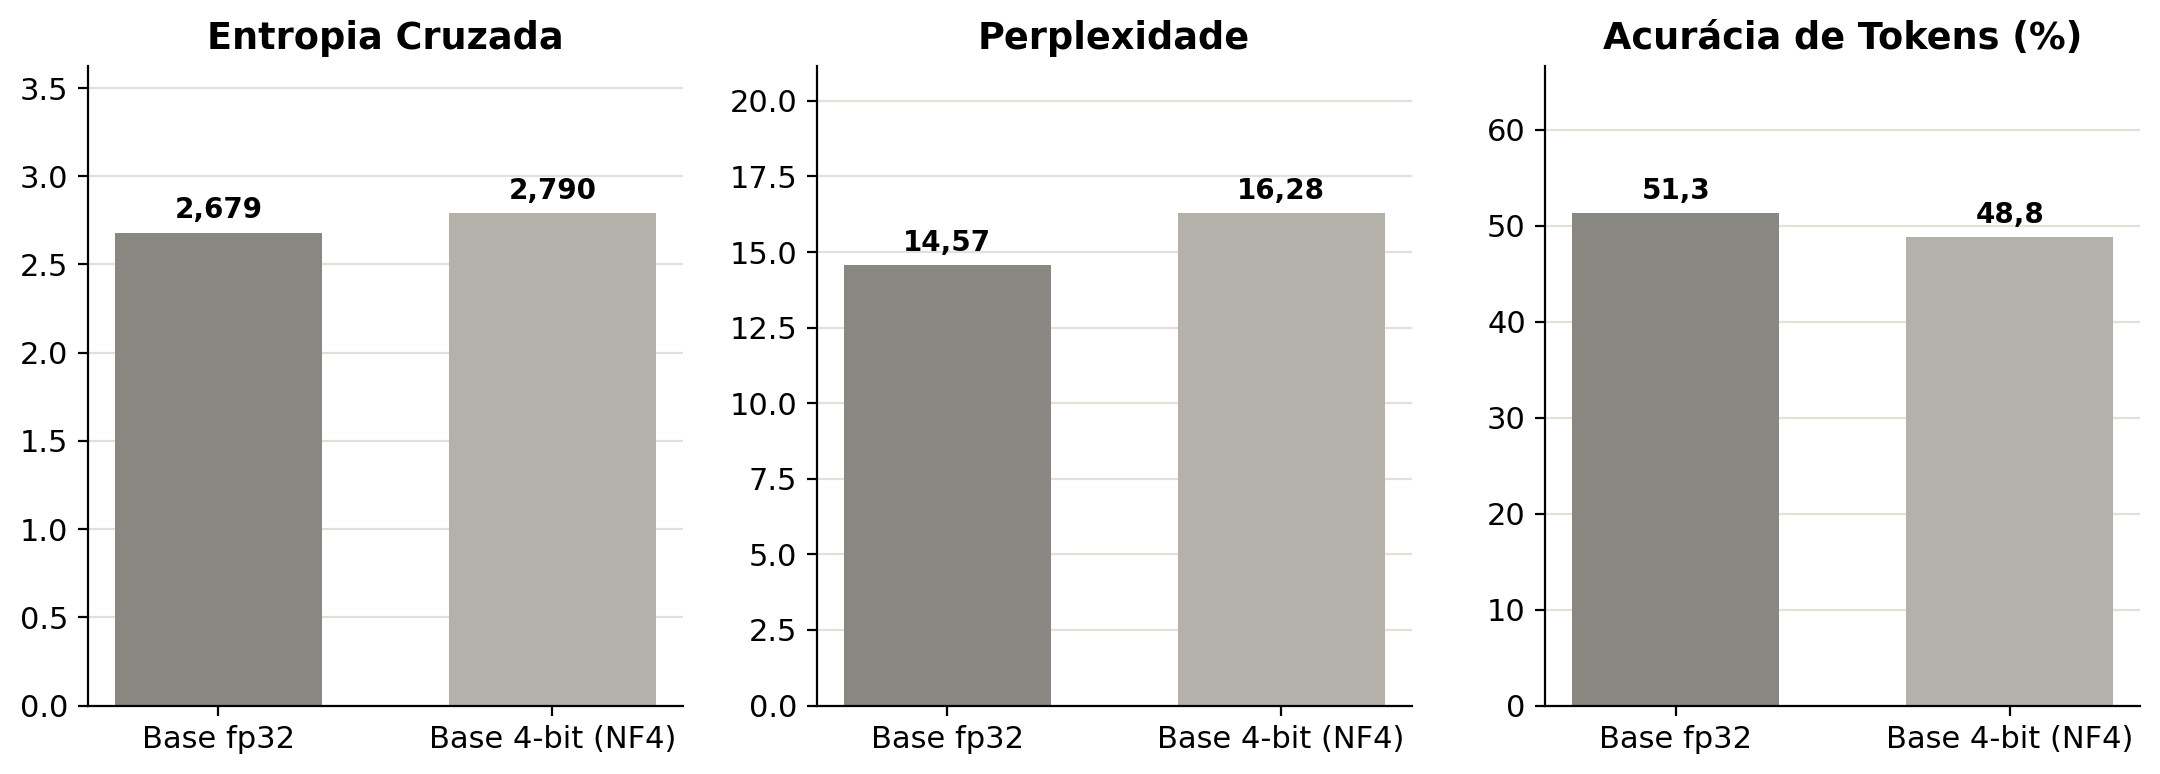
\includegraphics[width=\textwidth]{q3_quantizacao.png}
    \column{0.46\textwidth}
      \begin{itemize}
        \item Base quantizada em 4 bits (NF4); adaptadores de posto 16 nas projeções de atenção
        \item Mesmos dados, split, máscara e lote da Q2: comparação justa
        \item Preço da quantização no baseline: perplexidade de 14,57 para 16,28 (+11,7\%)
        \item Adaptador final: \textbf{8,7 MB} (contra $\approx$1 GB do modelo completo)
      \end{itemize}
  \end{columns}
\end{frame}

\begin{frame}{Q3: QLoRA contra SFT completo}
  \begin{columns}[c]
    \column{0.55\textwidth}
      \begin{center}
        
\includegraphics[height=0.82\textheight]{q3_painel_comparativo.png}
      \end{center}
    \column{0.43\textwidth}
      \begin{itemize}
        \item Perplexidade final \textbf{menor} que a do SFT completo (6,40 contra 7,49) partindo de baseline pior
        \item 228 vezes menos parâmetros treinados, 5,5 vezes menos VRAM
        \item Explicação: o adaptador de baixo posto regulariza; a validação do QLoRA caiu monotonicamente enquanto o SFT completo overfitou
      \end{itemize}
  \end{columns}
\end{frame}

\begin{frame}{O achado central: eficiência contra memorização}
  \begin{columns}[T]
    \column{0.48\textwidth}
      \textbf{Pela perplexidade}
      \begin{itemize}
        \item QLoRA 0.5B: \depois{6,40}
        \item SFT completo: 7,49
      \end{itemize}
      \vspace{0.5em}
      \textbf{Pelos fatos (10 perguntas)}
      \begin{itemize}
        \item SFT completo: \depois{6 acertos}
        \item QLoRA 0.5B: \alert{2 acertos}
      \end{itemize}
    \column{0.5\textwidth}
      \textbf{Leitura}
      \begin{itemize}
        \item Atualizar todos os pesos memoriza fatos novos com mais força
        \item O adaptador aprende formato e distribuição, mas retém menos fatos no 0.5B
        \item \textbf{Saída prática:} QLoRA no 1.5B recupera os fatos (5 de 10) com perplexidade 4,75 em 2,75 GB
      \end{itemize}
  \end{columns}
  \vfill
  \begin{exampleblock}{Conclusão da comparação}
    Sob restrição de memória, vale mais adaptar eficientemente um modelo maior do que ajustar completamente um modelo menor.
  \end{exampleblock}
\end{frame}

\begin{frame}{Visão consolidada das Questões 01 a 03}
  \begin{center}
    
\includegraphics[width=0.98\textwidth]{resumo_geral.png}
  \end{center}
\end{frame}

\section{Questão 04: Destilação de Conhecimento}

\begin{frame}{Q4: destilação por Chain-of-Thought (3B $\to$ 1.5B)}
  \begin{columns}[T]
    \column{0.46\textwidth}
      \begin{itemize}
        \item Professor \textbf{Qwen2.5-3B} gera raciocínio e resposta; aluno \textbf{Qwen2.5-1.5B} aprende por LoRA
        \item Dataset sintético do DOMPI-2025 (100 trechos)
        \item Avaliação: \textit{benchmark} de 100 perguntas mais métricas quantitativas
      \end{itemize}
    \column{0.52\textwidth}
      \small
      \begin{tabular}{@{}l c c@{}}
        \toprule
        & \textbf{PPL} & \textbf{Acc. tokens} \\
        \midrule
        Professor 3B          & 4,50 & 68,08\% \\
        \antes{Aluno antes}    & 5,49 & 65,65\% \\
        \depois{Aluno depois}  & \textbf{4,23} & \textbf{68,65\%} \\
        \bottomrule
      \end{tabular}
      \vspace{0.8em}

      Perplexidade do aluno de \antes{5,49} para \depois{4,23} (queda de 22,9\%); no domínio, o aluno até supera o professor.
  \end{columns}
\end{frame}

\begin{frame}{Q4: dois avaliadores, conclusões opostas}
  \begin{columns}[T]
    \column{0.48\textwidth}
      \small
      \begin{tabular}{@{}l c c@{}}
        \toprule
        \textbf{Método} & \textbf{Antes} & \textbf{Depois} \\
        \midrule
        \textit{Substring}    & 36\% & \depois{42\%} \\
        \textit{LLM-as-Judge} & \alert{69\%} & 62\% \\
        \bottomrule
      \end{tabular}
    \column{0.52\textwidth}
      \begin{itemize}
        \item Pela correspondência textual, o aluno \depois{melhora} ($+6$ pp)
        \item Pelo juiz semântico, o aluno \alert{piora} ($-7$ pp): o ajuste aproximou o formato, mas introduziu alucinações
      \end{itemize}
  \end{columns}
  \vfill
  \begin{alertblock}{Lição}
    Menor perplexidade não implica respostas mais confiáveis: a métrica escolhida pode inverter a conclusão sobre a destilação.
  \end{alertblock}
\end{frame}

\section{Questão 05: RAG}

\begin{frame}{Q5: RAG sobre o docentesDC reduz alucinações}
  \begin{columns}[T]
    \column{0.5\textwidth}
      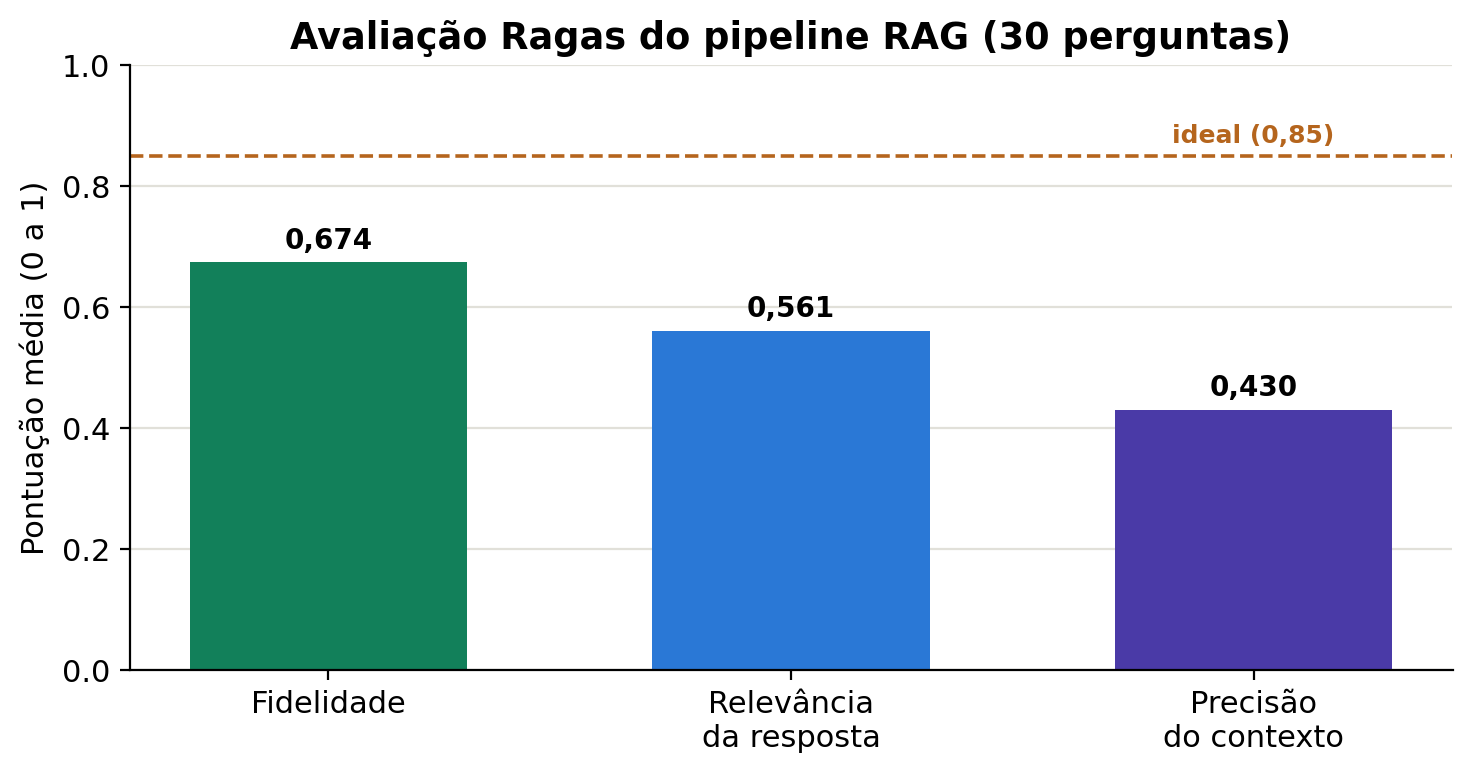
\includegraphics[width=\textwidth]{q5_ragas.png}
    \column{0.5\textwidth}
      \begin{itemize}
        \item \textbf{Standard RAG}: LangChain + ChromaDB + \texttt{gpt-4o-mini}
        \item Avaliação Ragas em 30 perguntas: fidelidade 0,67, relevância 0,56, precisão 0,43
        \item Notas baixas vêm de lacunas do \textit{benchmark}, não do pipeline
      \end{itemize}
  \end{columns}
  \vfill
  \begin{exampleblock}{Contribuição do RAG}
    Sem contexto, o modelo inventa ou recusa; com RAG, cita o material real ou admite honestamente ``não encontrei essa informação no contexto''.
  \end{exampleblock}
\end{frame}

\section{Questão 06: Guardrails}

\begin{frame}{Q6: guardrails sobre o modelo da Questão 02}
  \begin{columns}[T]
    \column{0.56\textwidth}
      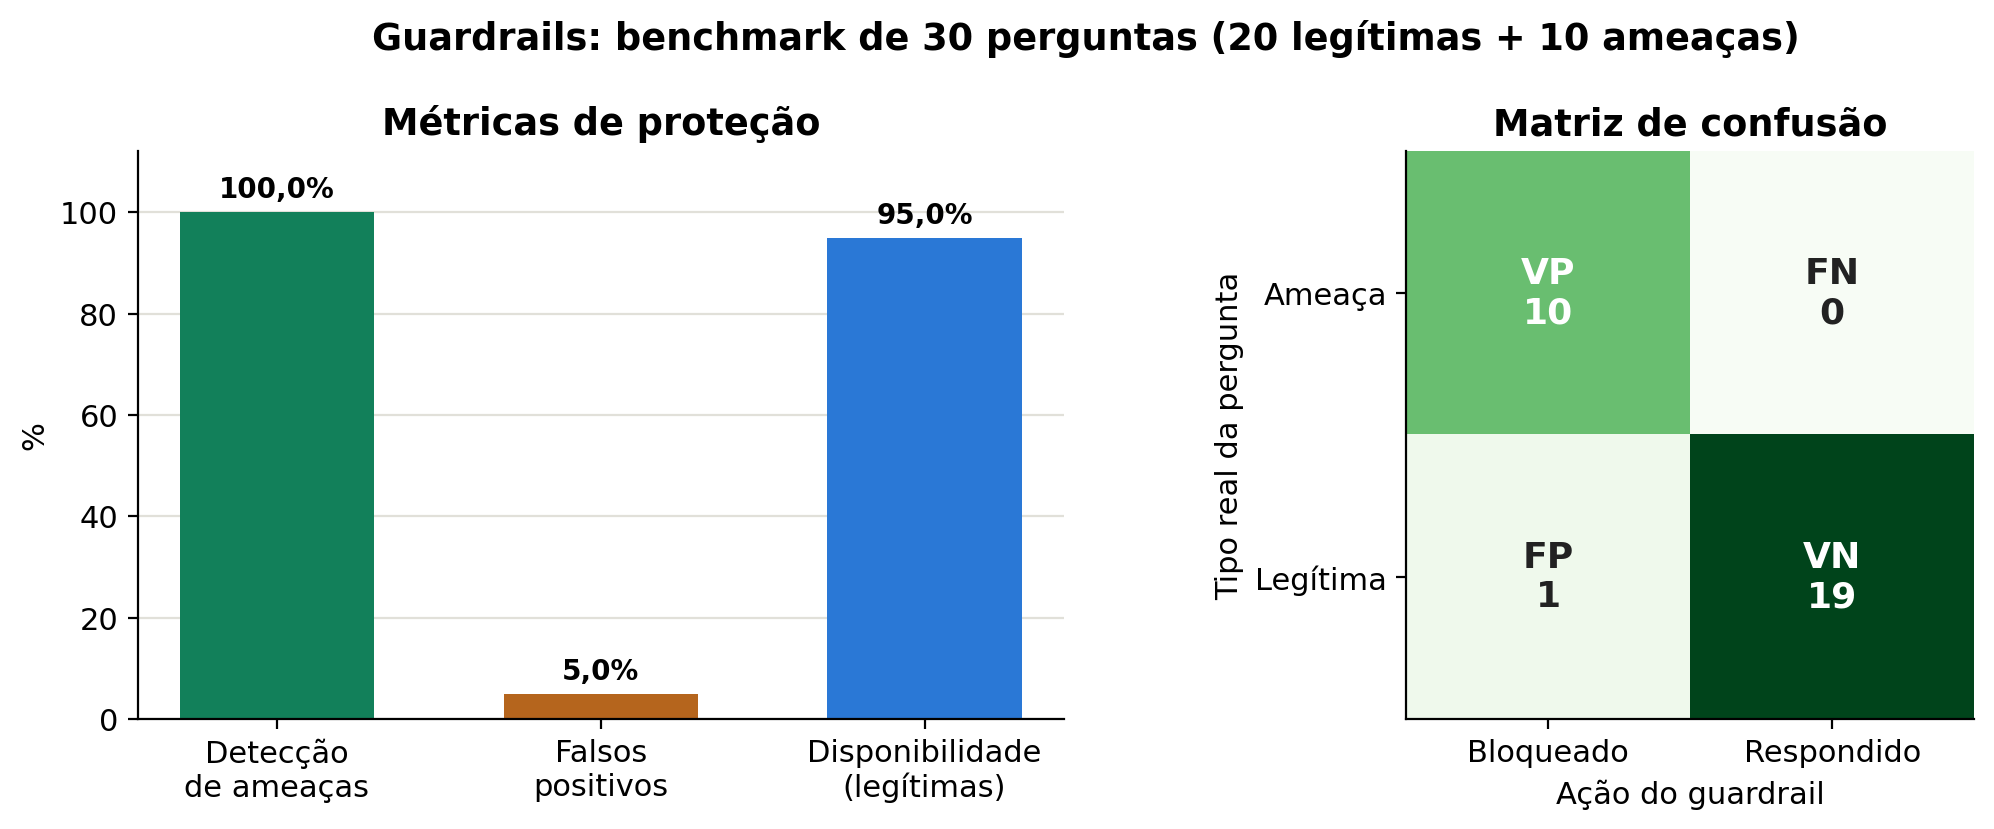
\includegraphics[width=\textwidth]{q6_guardrails.png}
    \column{0.42\textwidth}
      \begin{itemize}
        \item Três trilhos sobre o \textbf{Qwen2.5-0.5B} SFT: entrada, tópico e saída
        \item \textit{Benchmark} de 30 (20 legítimas + 10 ameaças)
        \item \depois{100\%} das ameaças bloqueadas, \depois{5\%} de falsos positivos, \depois{95\%} de disponibilidade
      \end{itemize}
  \end{columns}
  \vfill
  Sem \textit{guardrails}, o modelo respondia a tudo, inclusive instruções nocivas: a exposição a ameaças caiu a zero, com custo mínimo de disponibilidade.
\end{frame}

\section{Conclusões}

\begin{frame}{Conclusões}
  \small
  \begin{itemize}
    \item \textbf{Q1:} o pré-treino continuado adaptou o modelo ao domínio (perplexidade 90\% menor) e memorizou fatos exatos do corpus, com o risco novo de alucinações plausíveis
    \item \textbf{Q2:} um pipeline de dados programático viabilizou SFT eficaz e honesto, com overfitting neutralizado pela seleção de checkpoint
    \item \textbf{Q3:} QLoRA entregou a melhor perplexidade a uma fração do custo, com trade-off na retenção factual
    \item \textbf{Q4:} a destilação transferiu conhecimento nas métricas, mas o juiz semântico expôs alucinações
    \item \textbf{Q5:} o RAG trocou alucinação por citação do material real ou recusa honesta
    \item \textbf{Q6:} os guardrails bloquearam 100\% das ameaças com 5\% de falsos positivos
  \end{itemize}
  \vfill
  \begin{exampleblock}{Arco do trabalho}
    Adaptar (Q1--Q3), comprimir preservando conhecimento (Q4), complementar com recuperação (Q5) e proteger no uso (Q6).
  \end{exampleblock}
\end{frame}

\begin{frame}[standout]
  Obrigado! \\ \vspace{0.5em} {\small Perguntas?}
\end{frame}

\end{document}
